\documentclass[11pt]{article}

\usepackage{graphicx}
\usepackage{caption}

\marginparwidth 0.5in 
\oddsidemargin 0.25in 
\evensidemargin 0.25in 
\marginparsep 0.25in
\topmargin 0.0in 
\textwidth 6in \textheight 8.5in

\title{sQuire: A Web Based Collaborative Editor\\Homework 6 Individual Work\\Group 3}
\author{Rick Boss (boss2849)}

\begin{document}
\maketitle

\subsection{Create Project (boss2849)}
\begin{minipage}{1\textwidth}
    \begin{center}
    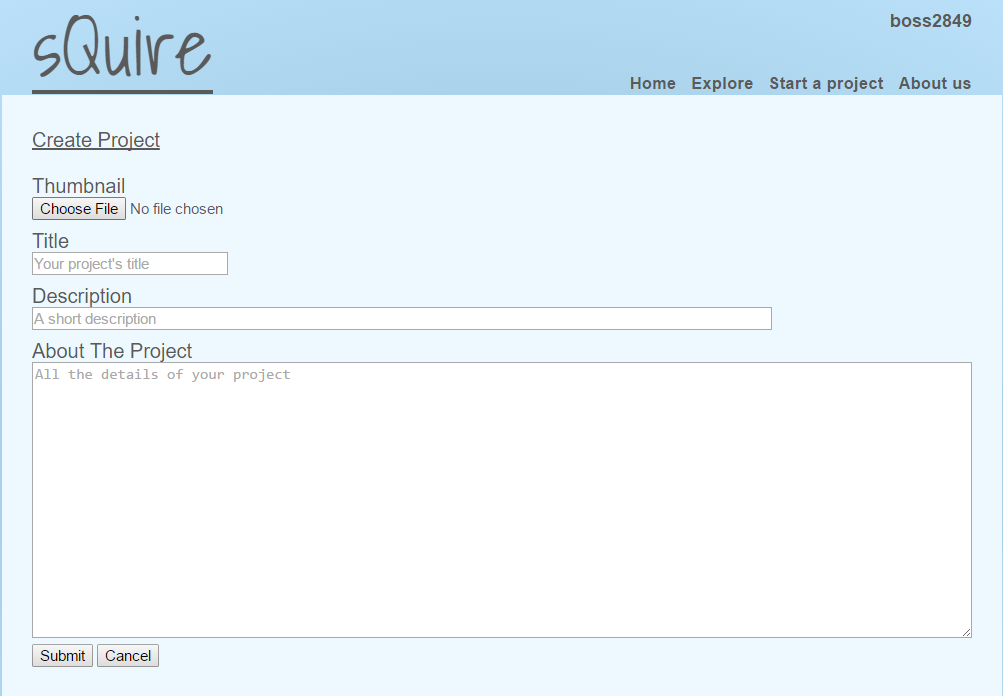
\includegraphics[width=0.9\textwidth]{protos/proto-createproject-boss2849}
    \end{center}
    \caption{figure}{The create project page was made for users to submit new project ideas. It allows them to upload a thumbnail, add a short description (used in brief views of the project) and a full project description. Submitting will create a new project and take the user to that page.}
\end{minipage}

\subsection{View Project (boss2849)}
\begin{minipage}{1\textwidth}
    \begin{center}
    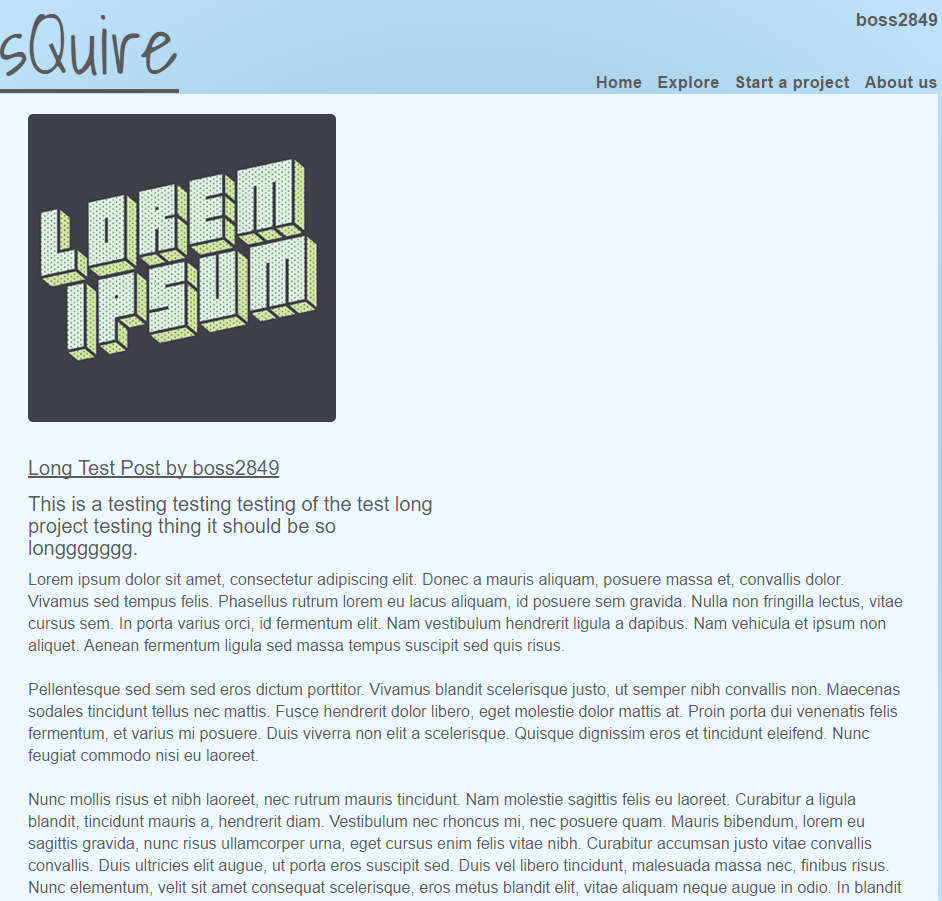
\includegraphics[width=0.9\textwidth]{protos/proto-viewproject-boss2849}
    \end{center}
    \caption{figure}{Each project will have a page dedicated just to the description of the project. Here other users can see the main project image, a short description, and the full explanation of the project.}
\end{minipage}

\end{document}
